\documentclass[10pt]{article}
\usepackage[a4paper,margin=0.65in]{geometry}
\usepackage{amsmath,amssymb}
\usepackage{booktabs}
\usepackage{graphicx}
\usepackage{placeins}
\usepackage{float}
\graphicspath{{./}}

\title{Gabor Vector-Field Model Comparison with Fixed Hyperparameter Sweeps}
\author{Rishabh Kumar}
\date{\today}

\begin{document}
\maketitle

\begin{abstract}
This report compares parametric spiral families and non-parametric kernel/RKHS families on the Gabor-filter vector-field exports in \texttt{vf\_exports}.  Unlike the earlier adaptive-grid analysis, every kernel model here uses the same broad fixed hyperparameter grids.  The primary score is held-out axial residual sum of squares (RSS), not Bayesian evidence.  The plots overlay fitted streamlines on the original Gabor arrows, with the observed field drawn at opacity $\alpha=0.7$.
\end{abstract}

\section{Data and Angular Representation}
Each Gabor CSV row supplies a coordinate $(x_i,y_i)$ and the local pitch angle $\alpha'_i$ in degrees.  Because $\alpha'_i$ is not the global field direction, the observed modelling angle is reconstructed as
\[
  \phi_i=\operatorname{atan2}(y_i,x_i)+\alpha'_i.
\]
The models are scored as line fields, so $\phi$ and $\phi+\pi$ are equivalent.  Held-out error uses the axial residual
\[
  \Delta_i=\frac12\operatorname{atan2}\left(\sin 2(\phi_i-\hat\phi_i),\cos 2(\phi_i-\hat\phi_i)\right).
\]
The reported RSS is the mean across shuffled 10-fold cross-validation folds of the per-held-out-point sum $\sum_i\Delta_i^2/|I_k|$.

\section{Fixed Hyperparameter Sweep}
The kernel sweep is intentionally wide and fixed across datasets.  It does not use the dataset-adaptive length-scale or noise ranges from the earlier analysis.

\begin{center}
\begin{tabular}{lrrrr}
\toprule
Hyperparameter & Count & Min & Max & Grid \\
\midrule
bandwidth\_or\_radius\_ell & 72 & 1 & 1.5e+03 & geomspace \\
sigma\_n & 17 & 0.001 & 10 & geomspace \\
kappa & 19 & 0 & 64 & explicit \\
parametric\_fixed\_p & 3 & 0 & 2 & \{0,1,2\} \\
parametric\_continuous\_p\_bounds &  & -0.999 & 2.999 & L-BFGS-B bounds \\
parametric\_gamma\_bounds &  & -3.141593 & 3.141593 & L-BFGS-B bounds \\
\bottomrule
\end{tabular}
\end{center}

The Gaussian RBF and uniform kernels each evaluate $72\times17=1224$ kernel--noise settings per dataset.  The multiplicative RBF--von-Mises kernel evaluates $72\times17\times19=23256$ settings per dataset.  Each setting is scored by shuffled 10-fold held-out axial RSS with random seed 42.

\section{Model Families}
The non-parametric families are Gaussian RBF, uniform local-neighbourhood, and multiplicative RBF--von-Mises kernels on the doubled-angle embedding $(\cos 2\phi,\sin 2\phi)$.  The parametric families are fixed $p\in\{0,1,2\}$ and a continuous $p$ family with $p\in[-0.999,2.999]$ and $\gamma\in[-\pi,\pi]$.

\section{Results}
\subsection{Winner Counts}
\begin{center}
\begin{tabular}{lr}
\toprule
Model & Wins \\
\midrule
Multiplicative RBF-VM RKHS & 6 \\
Gaussian RBF RKHS & 2 \\
Uniform RKHS & 2 \\
\bottomrule
\end{tabular}
\end{center}

\subsection{Held-Out RSS Summary}
\begin{center}
\begin{tabular}{lrrrr}
\toprule
Model & Datasets & Mean RSS & Median RSS & Mean MAE deg \\
\midrule
Multiplicative RBF-VM RKHS & 10 & 0.3396 & 0.3358 & 24.7723 \\
Gaussian RBF RKHS & 10 & 0.342 & 0.3417 & 24.8753 \\
Uniform RKHS & 10 & 0.3576 & 0.3488 & 25.8737 \\
Parametric p=0 (Logarithmic) & 10 & 0.7851 & 0.78 & 43.843 \\
Parametric p=1 (Archimedean) & 10 & 0.7986 & 0.7736 & 43.964 \\
Parametric continuous p & 10 & 0.8045 & 0.8138 & 44.3255 \\
Parametric p=2 (Fermat) & 10 & 0.8278 & 0.8407 & 44.8518 \\
\bottomrule
\end{tabular}
\end{center}

\subsection{Selected Kernel Hyperparameters}
\begin{center}
\begin{tabular}{lrrrrrrrrr}
\toprule
Model & $\ell$ min & $\ell$ med & $\ell$ max & $\sigma_n$ min & $\sigma_n$ med & $\sigma_n$ max & $\kappa$ min & $\kappa$ med & $\kappa$ max \\
\midrule
Gaussian RBF RKHS & 24.3637 & 50.3709 & 103.0423 & 0.001 & 0.5623 & 10 &  &  &  \\
Multiplicative RBF-VM RKHS & 24.3637 & 52.8229 & 319.9529 & 0.0178 & 1 & 3.1623 & 0 & 0.625 & 3 \\
Uniform RKHS & 45.2008 & 58.5539 & 68.2466 & 0.0562 & 5.6234 & 10 &  &  &  \\
\bottomrule
\end{tabular}
\end{center}

\subsection{Dataset Winners}
\begin{center}
\begin{tabular}{lrrr}
\toprule
Dataset & Winner & RSS & MAE deg \\
\midrule
Front\_EE-1\_1\_3000x\_rings\_coords.csv & Multiplicative RBF-VM RKHS & 0.2587 & 20.7635 \\
Front\_EE-1\_2\_3000x\_rings\_coords.csv & Multiplicative RBF-VM RKHS & 0.2194 & 18.4802 \\
Front\_EE-1\_3\_3000x\_rings\_coords.csv & Gaussian RBF RKHS & 0.4909 & 31.8122 \\
Front\_EE-1\_4\_3000x\_rings\_coords.csv & Gaussian RBF RKHS & 0.388 & 27.623 \\
Front\_EE-1\_5\_3000x\_rings\_coords.csv & Multiplicative RBF-VM RKHS & 0.34 & 24.4879 \\
Front\_EE1\_1\_3000x\_rings\_coords.csv & Multiplicative RBF-VM RKHS & 0.15 & 16.0471 \\
Front\_EE1\_2\_3000x\_rings\_coords.csv & Uniform RKHS & 0.4622 & 29.9347 \\
Front\_EE1\_3\_3000x\_rings\_coords.csv & Uniform RKHS & 0.3312 & 25.0436 \\
Front\_EE1\_4\_3000x\_rings\_coords.csv & Multiplicative RBF-VM RKHS & 0.2572 & 22.3987 \\
Front\_EE1\_5\_3000x\_rings\_coords.csv & Multiplicative RBF-VM RKHS & 0.4834 & 30.8891 \\
\bottomrule
\end{tabular}
\end{center}

\begin{figure}[H]
\centering
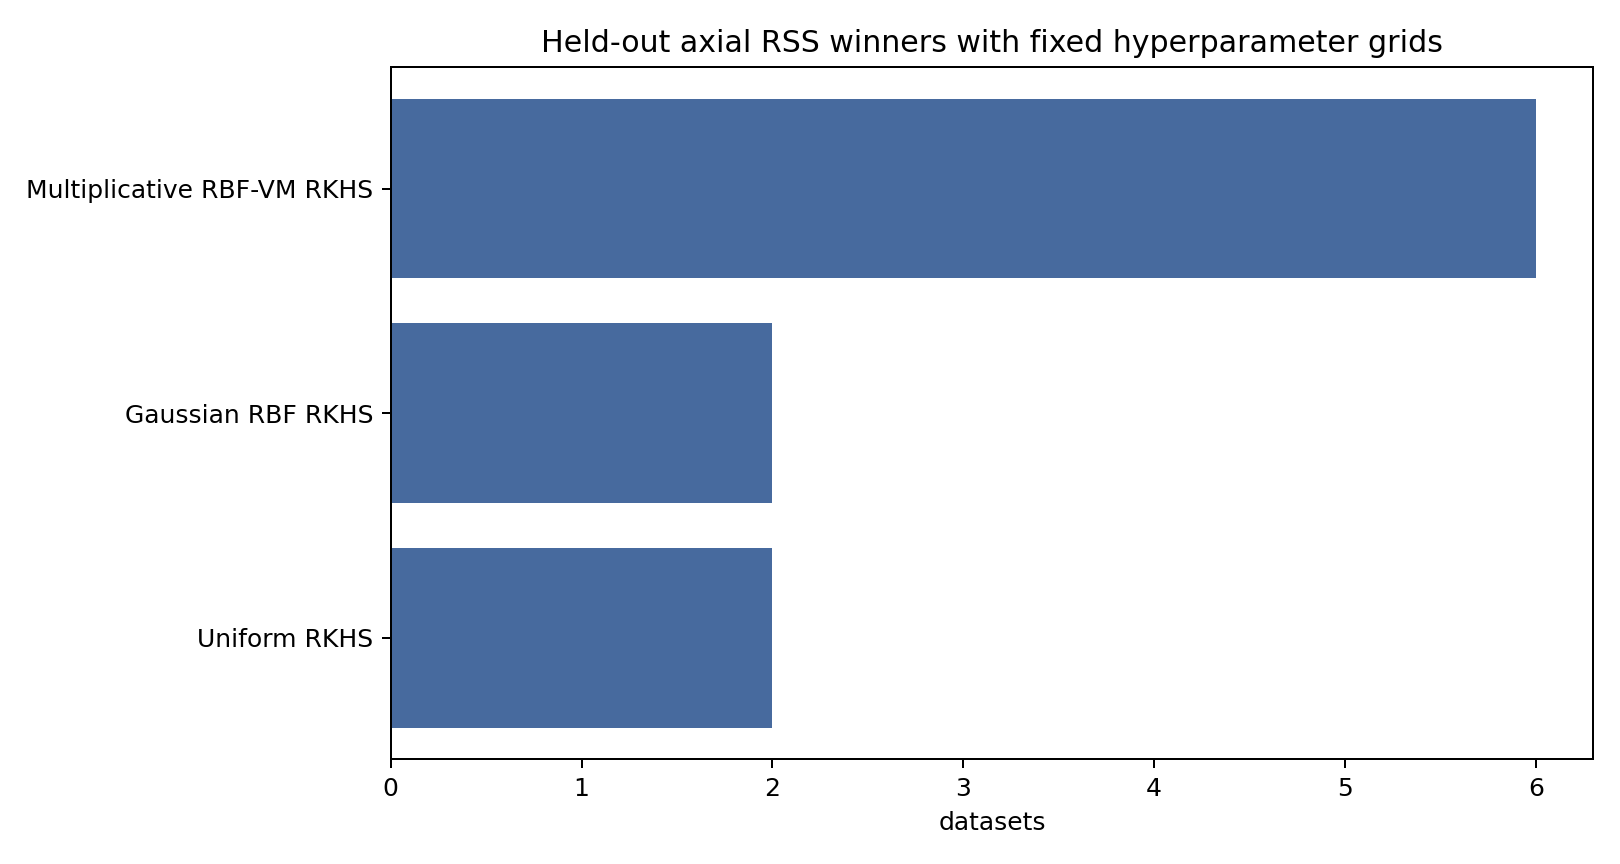
\includegraphics[width=0.82\linewidth]{plots/winner_counts_fixed_grid.png}
\caption{Winner counts under the fixed-grid held-out RSS comparison.}
\end{figure}

\begin{figure}[H]
\centering
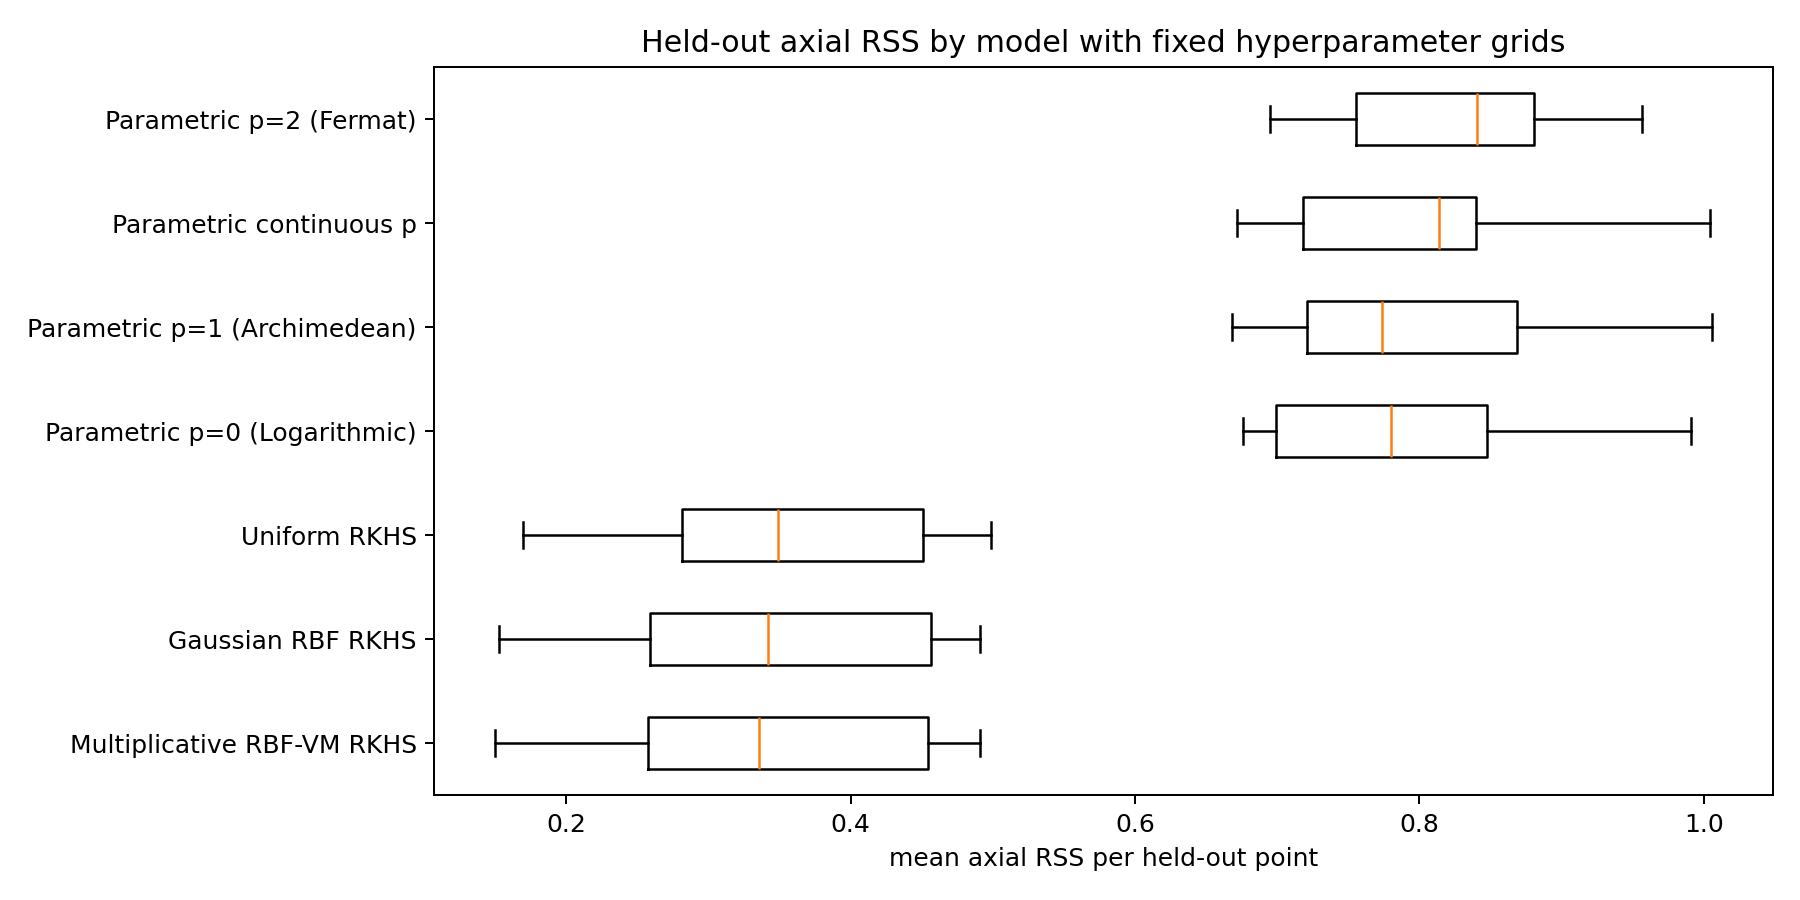
\includegraphics[width=0.86\linewidth]{plots/cv_axial_rss_boxplot_fixed_grid.png}
\caption{Distribution of held-out axial RSS across the 10 Gabor datasets.}
\end{figure}

\FloatBarrier

\section{Fitted Overlay Plots}
Each plot shows the original Gabor vector field and the fitted streamlines for all compared families.  The Gabor arrows come from $\alpha'$ after conversion to the global angle $\phi=\operatorname{atan2}(y,x)+\alpha'$.

\begin{figure}[p]
\centering
\includegraphics[width=\linewidth]{plots/fitted\_overlays/Front\_EE-1\_1\_3000x\_rings\_coords\_fixed\_grid\_overlays.png}
\caption{Fitted overlays for \texttt{Front\_EE-1\_1\_3000x\_rings\_coords.csv}.  The observed Gabor field is shown with arrow opacity $\alpha=0.7$; fitted models are shown as streamlines.}
\end{figure}
\begin{figure}[p]
\centering
\includegraphics[width=\linewidth]{plots/fitted\_overlays/Front\_EE-1\_2\_3000x\_rings\_coords\_fixed\_grid\_overlays.png}
\caption{Fitted overlays for \texttt{Front\_EE-1\_2\_3000x\_rings\_coords.csv}.  The observed Gabor field is shown with arrow opacity $\alpha=0.7$; fitted models are shown as streamlines.}
\end{figure}
\begin{figure}[p]
\centering
\includegraphics[width=\linewidth]{plots/fitted\_overlays/Front\_EE-1\_3\_3000x\_rings\_coords\_fixed\_grid\_overlays.png}
\caption{Fitted overlays for \texttt{Front\_EE-1\_3\_3000x\_rings\_coords.csv}.  The observed Gabor field is shown with arrow opacity $\alpha=0.7$; fitted models are shown as streamlines.}
\end{figure}
\begin{figure}[p]
\centering
\includegraphics[width=\linewidth]{plots/fitted\_overlays/Front\_EE-1\_4\_3000x\_rings\_coords\_fixed\_grid\_overlays.png}
\caption{Fitted overlays for \texttt{Front\_EE-1\_4\_3000x\_rings\_coords.csv}.  The observed Gabor field is shown with arrow opacity $\alpha=0.7$; fitted models are shown as streamlines.}
\end{figure}
\begin{figure}[p]
\centering
\includegraphics[width=\linewidth]{plots/fitted\_overlays/Front\_EE-1\_5\_3000x\_rings\_coords\_fixed\_grid\_overlays.png}
\caption{Fitted overlays for \texttt{Front\_EE-1\_5\_3000x\_rings\_coords.csv}.  The observed Gabor field is shown with arrow opacity $\alpha=0.7$; fitted models are shown as streamlines.}
\end{figure}
\begin{figure}[p]
\centering
\includegraphics[width=\linewidth]{plots/fitted\_overlays/Front\_EE1\_1\_3000x\_rings\_coords\_fixed\_grid\_overlays.png}
\caption{Fitted overlays for \texttt{Front\_EE1\_1\_3000x\_rings\_coords.csv}.  The observed Gabor field is shown with arrow opacity $\alpha=0.7$; fitted models are shown as streamlines.}
\end{figure}
\begin{figure}[p]
\centering
\includegraphics[width=\linewidth]{plots/fitted\_overlays/Front\_EE1\_2\_3000x\_rings\_coords\_fixed\_grid\_overlays.png}
\caption{Fitted overlays for \texttt{Front\_EE1\_2\_3000x\_rings\_coords.csv}.  The observed Gabor field is shown with arrow opacity $\alpha=0.7$; fitted models are shown as streamlines.}
\end{figure}
\begin{figure}[p]
\centering
\includegraphics[width=\linewidth]{plots/fitted\_overlays/Front\_EE1\_3\_3000x\_rings\_coords\_fixed\_grid\_overlays.png}
\caption{Fitted overlays for \texttt{Front\_EE1\_3\_3000x\_rings\_coords.csv}.  The observed Gabor field is shown with arrow opacity $\alpha=0.7$; fitted models are shown as streamlines.}
\end{figure}
\begin{figure}[p]
\centering
\includegraphics[width=\linewidth]{plots/fitted\_overlays/Front\_EE1\_4\_3000x\_rings\_coords\_fixed\_grid\_overlays.png}
\caption{Fitted overlays for \texttt{Front\_EE1\_4\_3000x\_rings\_coords.csv}.  The observed Gabor field is shown with arrow opacity $\alpha=0.7$; fitted models are shown as streamlines.}
\end{figure}
\begin{figure}[p]
\centering
\includegraphics[width=\linewidth]{plots/fitted\_overlays/Front\_EE1\_5\_3000x\_rings\_coords\_fixed\_grid\_overlays.png}
\caption{Fitted overlays for \texttt{Front\_EE1\_5\_3000x\_rings\_coords.csv}.  The observed Gabor field is shown with arrow opacity $\alpha=0.7$; fitted models are shown as streamlines.}
\end{figure}

\FloatBarrier

\section{Interpretation}
The fixed-grid rerun confirms the qualitative conclusion from held-out RSS: the kernel families fit the Gabor vector-field exports substantially better than the current parametric spiral families.  With the wider and denser non-adaptive grid, the multiplicative RBF--von-Mises kernel has the best mean held-out RSS, with Gaussian RBF very close behind.  The parametric models remain interpretable, but their held-out axial errors are roughly twice as large.

\end{document}
